\section{Introduction}

Today's end-user mobile devices, such as smartphones and
tablets, have become indispensable gadgets in people's everyday
life, and thus have created increasing research opportunities.
As a result, the Internet architecture, end-user traffic
patterns, etc., have also evolved rapidly. These devices
generate useful information for service providers and policy
makers to enhance network research and the services provided.
These devices also provide a platform for researchers to
investigate how new applications can provide better performance.
As a result, there has been significant interests in the network
community to study mobile network and devices, and in the
systems community to deploy new services and test research
prototypes, such as Phonelab~\cite{nandugudi2013phonelab}, 
Mobilyzer~\cite{nikravesh2015mobilyzer}, etc.
					
For researchers, however, there are two obstacles for research
about mobile devices. First, the privacy and security challenges
have increased dramatically over the years. The use of 
smartphones and tablets has introduced a new class of threats. 
For example, a smartphone's GPS locations,
WiFi connections, or Bluetooth pairing history can be highly
personal; a malicious party could also potentially bypass a
device's security protections and gain access to user
privileges. In particular, some seemingly benign apps can be a 
source of companies or governments to access ordinary 
people's daily activities~\cite{AngryBirds}. 
We not only need to ensure the security of a device
so that researcher's code cannot inadvertently damage or
maliciously hack into the device, but also protect the privacy
of device owners so that the code cannot eavesdrop on phone
conversations or infer passwords.

Second, it is challenging for researchers to perform meaningful
research related to end users without compromising data privacy
and ethical merit. Currently, research institutions adopt an
institutional review board (IRB) approval process where a
formally designated committee reviews, approves, and monitors
research involving human subjects~\cite{irb}.
Due to the different goals and unforeseen risks of each
individual project, the researcher needs to recruit subjects for
each research study, obtain their informed consent, etc. This
process is time-consuming, and the researcher needs to repeat
the process for every different projects. Even with the
recruited participants, the researchers from different research
groups cannot test their hypothesis at a world-wide scale or
reuse each other's user base.
					
This work is a first step towards lowering the technical
barriers to mobile Internet research without lowering the
ethical standard~\cite{zevenbergen2013ethical}, while 
protecting the security and privacy of end users. We design 
and implement Sensibility Testbed~\cite{sensibility, 
zhuang2014sensibility}, an Internet-wide measurement testbed for mobile devices that
allows researchers to run code and deploy services on ordinary
people's smartphones or tablets for research purpose. It ensures
the security of user-owned devices and the privacy of
user-generated data. First, the usage model of Sensibility Testbed is
unique in that it maintains testbed services to manage how device 
owners make their devices accessible to different research 
communities anonymously, without putting
their devices at risk. Meanwhile, it offers technical measures
that allow researchers to collect data from remote mobile
devices without impairing the device owner's privacy. The
Sensibility Testbed relieves researcher from the burden of
recruiting subjects for every single experiment; the device
owners need only give consents once, instead of giving multiple
consents to each project of each researcher.

\begin{figure}
\center{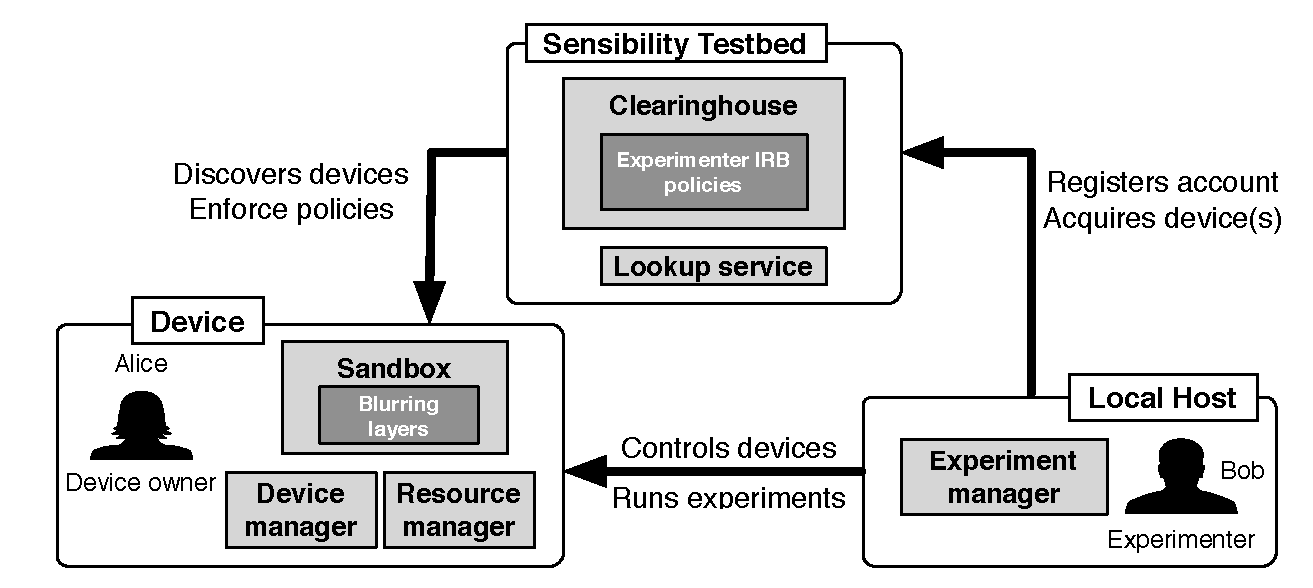
\includegraphics[width=\columnwidth]{figs/arch.pdf}}
%\vspace*{-20pt}
\caption{\small Sensibility Testbed architecture. \yanyan{need 
to replot this diagram.}
\label{fig-arch}}
\end{figure}

\textbf{Interacting parties.}
In Sensibility Testbed, there are three types of interacting
parties: mobile devices owned by ordinary people, with our app
installed; a clearinghouse server that discovers and configures
participating devices; and researchers wanting to run
experiments on mobile devices (see Figure~\ref{fig-arch}). Mobile devices
provide resources and data for researchers to use in their
experiments. In order to perform safe experiment on mobile
devices, a researcher must provide to the clearinghouse server
the IRB policies from his institute for accessing devices. These 
policies restrict what and how data can be accessed by the 
researcher. The
clearinghouse server helps the researcher acquire and manage
devices, and also codifies the policies specified by the
researcher's IRB into data blurring layers that are enforced on
mobile devices (Section XX). Such a process can protect device
owners' personal information. After obtaining remote sandboxes
and having IRB policies in place, researchers can perform
experiment on the devices using their credentials assigned by
the clearinghouse. Researchers' code runs in a sandbox on any
remote device that isolates the code from the rest of the device
host system. To control the execution of code, the researcher
uses a local machine to manage the experiments via an experiment
tool (ET). This tool can deploy and run experiments in sandboxes
on remote devices that are acquired through the clearinghouse.

\textbf{Enforcing IRB approved restrictions.}
A recent research study has shown that more than half of the 
surveyed individuals stated no problem in supplying imprecise 
data from their personal devices to protect their 
privacy~\cite{fawaz2014location}. Based on this fact, restricting 
the precision (spatial or temporal precision) or \textit{blurring 
data} would be a good privacy protection mechanism we can 
provide for end users. In Sensibility Testbed, the data blurring 
mechanism is implemented as reference monitors in sandbox, 
each enforcing an access control 
policy over sensor access~\cite{ref}. Using a sandboxing 
technique in our prior work~\cite{cappos2010retaining}, we can 
interject code to implement privacy policies and control what 
happens with the data gathered on the device. A sensor access 
policy can (1) reduce 
the precision of the raw sensor data returned from a device, such
as returning the device location at the city granularity; (2) restrict 
the frequency of accessing a sensor, such as the polling rate of 
accelerometer, to avoid password inferring; and (3) disable the 
access to a certain sensor in sensitive situations, such as 
turning off camera when a device is at residential or work areas.
\yanyan{we haven't implemented the last one.}

Using these techniques, Sensibility Testbed makes experiment
prototyping faster, the remote control and management of devices
easier, and running experiment code more secure. The
contributions of this work are as follows:

\begin{enumerate}
\item We design Sensibility Testbed, which uses security and 
privacy techniques to minimize the technical challenges for 
network researchers to perform meaningful research, without 
compromising ethical merit.

\item Sensibility Testbed supports generation of data access 
policies, specified by a researcher, and implementation of 
these policies on mobile devices to protect the privacy of 
device owners.

\item A consortium structure for minimizing the pain of IRB 
approvals.  This enables participants to opt in to a large 
array of very low risk experiments and for experimenters to 
get a blanket approval to work with that pool of participants.  
This eliminates the need for every experiment to get approval 
from every participant.\yanyan{not sure about this.}

\item \yanyan{Perhaps talk about IRB approved restrictions 
being technically enforced?  If so, perhaps roll it into the 
generation of policies.}
\end{enumerate}

The rest of this paper is organized as follows. 